\begin{multicols}{2}
	\item A empilhadeira manual tem uma massa de \SI{70}{\kilogram} e centro de massa em $G$. Se ela levanta a bobina de \SI{120}{\kilogram} com uma aceleração de $\SI{3}{\meter/\second^{2}}$, determine as reações em cada uma das quatro rodas. A carga é simétrica. Despreze a massa do braço móvel $CD$.
	
	\columnbreak
	
	\begin{flushright}
		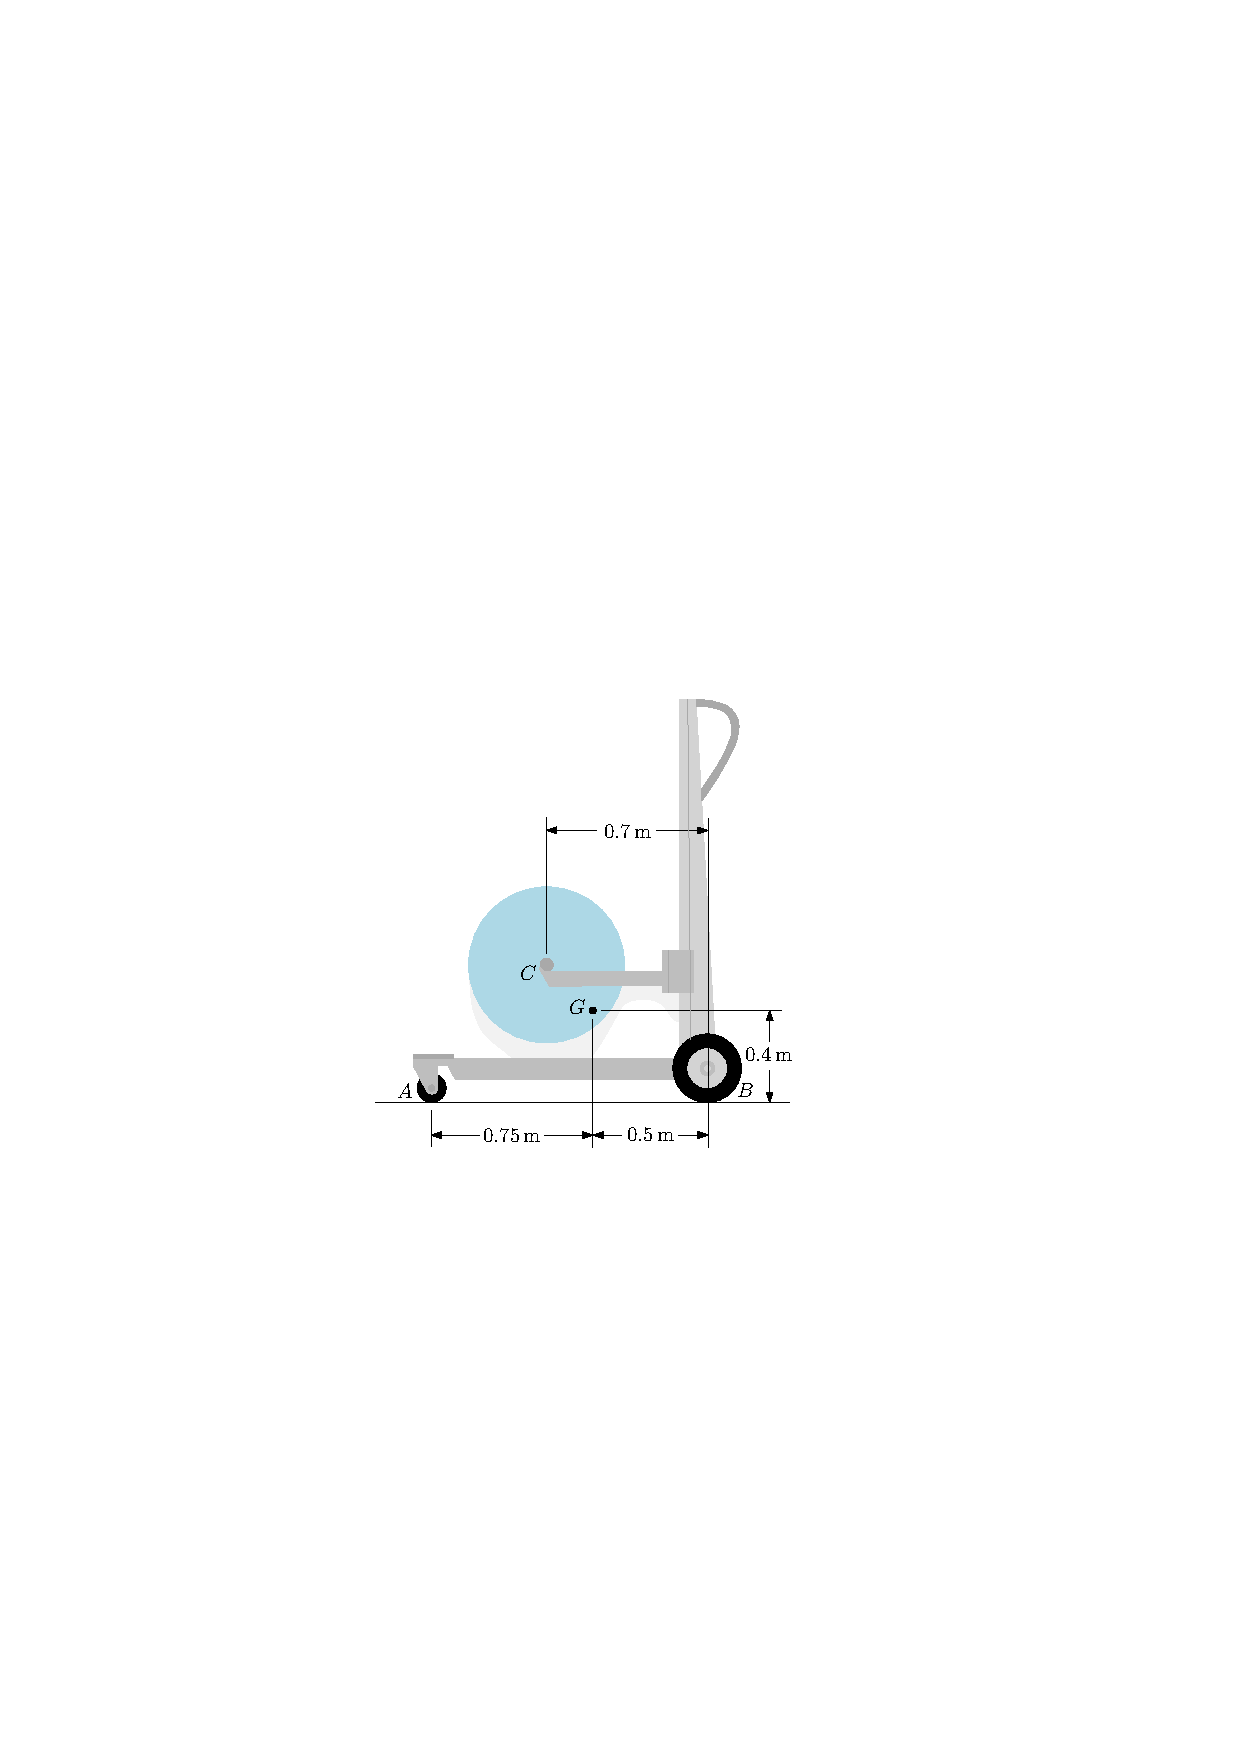
\includegraphics[scale=1.15]{../../images/draw_4}
	\end{flushright}
\end{multicols}